\section{Spring}

Spring is such a vast framework that it is worth its own section. 
In general the principle is as follows:

\begin{itemize}
    \item A main class starts the context. From the context, it starts the app.
    \item The context wires together all the loose beans of your model and your utils using a bean.xml
\end{itemize}

\subsection{Dependency injection}

A basic spring-app may be set up like this: 

\begin{lstlisting}[language=xml]
<dependencies>
	<dependency>
		<groupId>org.springframework</groupId>
		<artifactId>spring-context</artifactId>
		<version>4.3.10.RELEASE</version>
	</dependency>
</dependencies>
\end{lstlisting}

\begin{lstlisting}[language=java]
package model;

public interface Knight {
	public void embarkOnQuest();
}
\end{lstlisting}


\begin{lstlisting}[language=java]
package model;

public class BraveKnight implements Knight {

	private Quest quest;
	
	public BraveKnight(Quest quest) {
		this.quest = quest;
	}

	public void embarkOnQuest() {
		quest.embark();
	}
}
\end{lstlisting}


\begin{lstlisting}[language=java]
package model;

public interface Quest {
	public void embark();
}

\end{lstlisting}

\begin{lstlisting}[language=java]
package model;

public class DamselRescueQuest implements Quest {

	public void embark() {
		System.out.println("Knight will now rescue the damsel!");
	}

}
\end{lstlisting}


\begin{lstlisting}[language=java]
package model;

public class DragonSlayingQuest implements Quest {

	public void embark() {
		System.out.println("Knight will now slay the dragon!");
	}

}

\end{lstlisting}

\begin{lstlisting}[language=java]
package main;

import org.springframework.context.annotation.Bean;
import org.springframework.context.annotation.ComponentScan;
import org.springframework.context.annotation.Configuration;

import model.BraveKnight;
import model.DamselRescueQuest;
import model.Knight;
import model.Quest;

@Configuration
@ComponentScan("model")
public class KnightsConfig {

	@Bean
	public Knight knight() {
		return new BraveKnight(quest());
	}
	
	@Bean
	public Quest quest() {
		return new DamselRescueQuest();
	}
}
\end{lstlisting}


Annotations: 
\begin{itemize}
    \item Configuration: Use this class instead of a xml file for the wiring-instructions
    \item ComponentScan: look in these packages to scan for beans
    \item Bean: put this object in the spring context. By default, the bean will be given an ID that is the same as the @Bean-annotated method’s name.
\end{itemize}

\begin{lstlisting}[language=java]
package main;

import org.springframework.context.annotation.AnnotationConfigApplicationContext;

import model.Knight;

public class AppMain {

	public static void main(String[] args) {
		AnnotationConfigApplicationContext acac = new AnnotationConfigApplicationContext(KnightsConfig.class);
		
		Knight k = acac.getBean(Knight.class);
		k.embarkOnQuest();
		
		acac.close();
	}
}
\end{lstlisting}


As you can see, the basic idea is this: 
Use a DI framework to ensure that all beans are maximally decoupled and easily interchangeable.


\subsection{Aspects}

Aspects allow you to keep utility objects, like logging, authentication, security, etc out of your model. 

\begin{lstlisting}[language=xml]
<dependencies>
	<dependency>
		<groupId>org.springframework</groupId>
		<artifactId>spring-context</artifactId>
		<version>4.3.10.RELEASE</version>
	</dependency>

	<dependency>
		<groupId>org.springframework</groupId>
		<artifactId>spring-aop</artifactId>
		<version>4.3.10.RELEASE</version>
	</dependency>

	<dependency>
		<groupId>org.springframework</groupId>
		<artifactId>spring-aspects</artifactId>
		<version>4.3.10.RELEASE</version>
	</dependency>
</dependencies>
\end{lstlisting}

\begin{lstlisting}[language=java]
package util;

import java.io.PrintStream;

public class Minstrel {
	
	private PrintStream stream;

	public Minstrel(PrintStream stream) {
		this.stream = stream;
	}
	
	public void singBeforeQuest() {
		stream.println("Fa la la la, the knight is so brave!");
	}
	
	public void singAfterQuest() {
		stream.println("Tee hee hee, the brave knight did finish the quest!");
	}
}
\end{lstlisting}

\begin{lstlisting}[language=xml]
<?xml version="1.0" encoding="UTF-8"?>

<beans xmlns="http://www.springframework.org/schema/beans"
	xmlns:xsi="http://www.w3.org/2001/XMLSchema-instance" 
	xmlns:aop="http://www.springframework.org/schema/aop"
	xsi:schemaLocation="http://www.springframework.org/schema/aop
http://www.springframework.org/schema/aop/spring-aop-3.2.xsd
http://www.springframework.org/schema/beans
http://www.springframework.org/schema/beans/spring-beans.xsd">

	<bean id="knight" class="model.BraveKnight">
		<constructor-arg ref="quest"></constructor-arg>
	</bean>

	<bean id="quest" class="model.DamselRescueQuest">
	</bean>

	<bean id="minstrel" class="util.Minstrel">
		<constructor-arg value="#{T(System).out}"></constructor-arg>
	</bean>

	<aop:config>
		<aop:aspect ref="minstrel">
			<aop:pointcut id="embark" expression="execution(* *.embarkOnQuest(..))" />
			<aop:before pointcut-ref="embark" method="singBeforeQuest" />
			<aop:after pointcut-ref="embark" method="singAfterQuest" />
		</aop:aspect>
	</aop:config>

</beans>
\end{lstlisting}


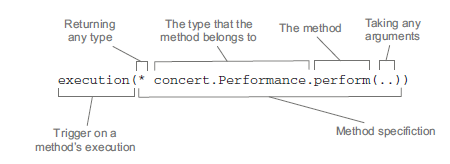
\includegraphics[width=8cm]{images/pointcut.png}

We put the knights.xml in src/main/resources. This is because files are loaded from the classpath, that is, the root of the produced jar. And resources is always put right into the root of the jar. 

\begin{lstlisting}[language=java]
package main;

import org.springframework.context.annotation.AnnotationConfigApplicationContext;
import org.springframework.context.support.ClassPathXmlApplicationContext;

import model.Knight;

public class AppMain {

	
	public static void main(String[] args) {
		ClassPathXmlApplicationContext ctx = new ClassPathXmlApplicationContext("knights.xml");

		Knight k = ctx.getBean(Knight.class);
		k.embarkOnQuest();
		
		ctx.close();
	}
}
\end{lstlisting}




Some jargon knowledge is in order:
\begin{itemize}
    \item advice: the action taken by an aspect. In the above example, \inlinecode{println}. Spring knows five kinds of advice: before, after, after-returning, after-throwing, and around.
    \item join-points: moments in the spring workflow where a advice may be applied. Internally, spring here loops through all registered aspects and checks if any of them applies in the given situation. (Equivalent to places where hooks are looped through in drupal.) In other words: any place in spring where \emph{some} aspect \emph{might} be applied. 
    \item pointcuts: a subset of all join-points, where \emph{an actual} aspect \emph{is} applied.
    \item introduction: An introduction allows you to add new methods or attributes to existing classes. For
    example, you could create an Auditable advice class that keeps the state of when an object was last modified. This could be as simple as having one method, setLast-Modified(Date), and an instance variable to hold this state. The new method and instance variable can then be introduced to existing classes without having to change them, giving them new behavior and state.
\end{itemize}

Aspects are woven in sometime during the execution of the application. Typically, an AOP container dynamically generates a proxy object that delegates to the target object while weaving in the aspects. This is how Spring AOP aspects are woven. However, JaspectJ can do this during compile-time!

You really don't need to use xml-configuration to be able to use aspects. We can also use the annotation-api borrowed from AspectJ: 

\begin{lstlisting}[language=java]
@Aspect
public class Audience {
	
	@Pointcut("execution(** concert.Performance.perform(..))")
	public void performance() {}

	@Before("performance()")
	public void silenceCellPhones() {
		System.out.println("Silencing cellphones");
	}
	
	@AfterThrowing("performance()")
	public void demandRefund() {
	System.out.println("Demanding a refund");
	}
}
\end{lstlisting}

Don't forget to tell spring that it should look for Aspects though!

\begin{lstlisting}[language=java]
@Configuration
@EnableAspectJAutoProxy
@ComponentScan
public class AppConfig {

	@Bean
	public Performance performance() {
		return new RollingStonesConcert();
	}
	
	@Bean
	public Audience audience() {
		return new Audience();
	}
}
\end{lstlisting}

\subsection{Templates}


\subsection{Bean lifecycle}
\begin{enumerate}
\item Spring instantiates the bean.
\item Spring injects values and bean references into the bean’s properties.
\item If the bean implements BeanNameAware, Spring passes the bean’s ID to the setBeanName() method.
\item If the bean implements BeanFactoryAware, Spring calls the setBeanFactory()
method, passing in the bean factory itself.
\item If the bean implements ApplicationContextAware, Spring calls the setApplicationContext() method, passing in a reference to the enclosing application
context.
\item If the bean implements the BeanPostProcessor interface, Spring calls its postProcessBeforeInitialization() method.
\item If the bean implements the InitializingBean interface, Spring calls its afterPropertiesSet() method. Similarly, if the bean was declared with an initmethod,
then the specified initialization method is called.
\item If the bean implements BeanPostProcessor, Spring calls its postProcessAfterInitialization() method.
\item At this point, the bean is ready to be used by the application and remains in the
application context until the application context is destroyed.
\item If the bean implements the DisposableBean interface, Spring calls its
destroy() method. Likewise, if the bean was declared with a destroy-method,
the specified method is called.
\end{enumerate}

By default, all beans in Spring are singletons.

\subsection{Wireing}

There are three ways of letting spring wire your components. 
\begin{enumerate}
\item Automatically using annotations. Pro: simple. Con: you cannot set @Component or @Autowire in external libraries.\marginpar{@Autowire is bad anyway, because it fails when there are more than one implementations to pick from. However, if there is only one implementation, then we don't need DI in the first place!}
\item With a Java @Configuration class. Pro: it's java. Con: You might be tempted to put business logic in the configuration. 
\item With xml. Pro: xml has one and only one purpose: config. Con: You cannot use any logic in your wireing.
\end{enumerate}


\subsection{Mocking}



\subsection{Spring MVC}

A spring-mvc app can be created in the same folder structure as any other eclipse java app.

The app consists really only of three parts: 
\begin{itemize}
    \item the servlet-container - usually a embeded tomcat. 
    \item the servlet, known as the dispatcher servlet
        \begin{itemize}
            \item configured with 
            \item redirects all requests to \inlinecode{@Controller}'s
        \end{itemize}
    \item the ContextLoaderListener
        \begin{itemize}
            \item reads the spring configuration-file
            \item creates spring-context
            \item creates web-application-context
        \end{itemize}
\end{itemize}

There are a few basic elements to every mvc-app: 

\begin{itemize}
    \item @Component: generic stereotype for any Spring-managed component
    \item @Repository: stereotype for persistence layer (jdbc, jpa, ...)
    \item @Service: stereotype for service layer (anything between controller and persistance layer)
    \item @Controller
\end{itemize}

Don't be afraid to use these annotations. Contrary to the general case, those mark classes that can only be part of a spring mvc app. It doesn't make sense to share them with other apps, so we might as well litter them with annotations.



\subsubsection{General structure}

Generally, every \inlinecode{@Controller} gets requests based on the rules defined in the \inlinecode{@RequestMapping}. The result of a request to a controller is always a string of a view-name. 

\subsubsection{Configuration}

\begin{itemize}
    \item AppInitializer: extends \inlinecode{AbstractAnnotationConfigDispatcherServletInitializer}. An alternative to the traditional web.xml file. Provides two configuration-classes: The servlet-config and the root-config. 
    
    \item Servlet-config: extends \inlinecode{WebMvcConfigurerAdapter}. The configuration for the servlet. 
    
    \item Root-config: the configuration for the backend, consisting of beans that are fully unaware of being used by a web-app. 
\end{itemize}

\subsubsection{Application: a minimal setup}

\begin{lstlisting}[language=xml,title=src/main/resources/appconfig]
<?xml version="1.0" encoding="UTF-8"?>

<beans xmlns="http://www.springframework.org/schema/beans"
       xmlns:xsi="http://www.w3.org/2001/XMLSchema-instance"
       xmlns:context="http://www.springframework.org/schema/context"
       xsi:schemaLocation="http://www.springframework.org/schema/beans
                           http://www.springframework.org/schema/beans/spring-beans.xsd
                           http://www.springframework.org/schema/context
                           http://www.springframework.org/schema/context/spring-context.xsd ">

    <context:component-scan base-package="sm" />

</beans>
\end{lstlisting}

\begin{lstlisting}[language=xml,title=src/main/resources/webconfig]
<?xml version="1.0" encoding="UTF-8"?>

<beans xmlns="http://www.springframework.org/schema/beans"
       xmlns:xsi="http://www.w3.org/2001/XMLSchema-instance"
       xmlns:context="http://www.springframework.org/schema/context"
       xmlns:mvc="http://www.springframework.org/schema/mvc"
       xsi:schemaLocation="http://www.springframework.org/schema/beans
                           http://www.springframework.org/schema/beans/spring-beans.xsd
                           http://www.springframework.org/schema/mvc
                           http://www.springframework.org/schema/mvc/spring-mvc.xsd
                           http://www.springframework.org/schema/context
                           http://www.springframework.org/schema/context/spring-context.xsd ">

	<context:component-scan base-package="sm" />

	<mvc:annotation-driven />
	<mvc:resources mapping="/resources/**" location="/resources/" />

	<bean class="org.springframework.web.servlet.view.InternalResourceViewResolver">
		<property name="viewClass" value="org.springframework.web.servlet.view.JstlView" />
		<property name="prefix" value="/WEB-INF/views/" />
		<property name="suffix" value=".jsp" />
	</bean>
	
</beans>
\end{lstlisting}

\begin{lstlisting}[language=xml,title=src/main/webapp/WEB-INF/web.xml]
<?xml version="1.0" encoding="UTF-8"?>

<web-app xmlns="http://xmlns.jcp.org/xml/ns/javaee"
         xmlns:xsi="http://www.w3.org/2001/XMLSchema-instance"
         xsi:schemaLocation="http://xmlns.jcp.org/xml/ns/javaee
                             http://xmlns.jcp.org/xml/ns/javaee/web-app_3_1.xsd" version="3.1">


    <context-param>
        <param-name>contextConfigLocation</param-name>
        <param-value>classpath:appconfig.xml</param-value>
    </context-param>

    <listener>
        <listener-class>org.springframework.web.context.ContextLoaderListener</listener-class>
    </listener>

    <servlet>
        <servlet-name>MyApp</servlet-name>
        <servlet-class>org.springframework.web.servlet.DispatcherServlet</servlet-class>
        <init-param>
            <param-name>contextConfigLocation</param-name>
            <param-value>classpath:webconfig.xml</param-value>
        </init-param>
        <load-on-startup>1</load-on-startup>
    </servlet>

    <servlet-mapping>
        <servlet-name>MyApp</servlet-name>
        <url-pattern>/</url-pattern>
    </servlet-mapping>

</web-app>
\end{lstlisting}


\begin{lstlisting}[language=java,title=src/main/java/sm/controller/AppMain.java]
package sm.controller;

import org.springframework.stereotype.Controller;
import org.springframework.ui.Model;
import org.springframework.web.bind.annotation.RequestMapping;
import org.springframework.web.bind.annotation.RequestMethod;

@Controller
@RequestMapping("/")
public class HomeController {

    @RequestMapping(method = RequestMethod.GET)
    public String index(Model model){
        model.addAttribute("message", "Spring MVC XML Config Example");
        return "index";
    }

}
\end{lstlisting}


\begin{lstlisting}[language=xml,title=src/main/webapp/WEB-INF/views/index.jsp]
<%@ page contentType="text/html;charset=UTF-8" language="java" %>
<html>
<head>
    <title>Spring MVC XML Configuration Example</title>
</head>
<body>
    ${message}
</body>
</html>
\end{lstlisting}

\subsubsection{Application: what goes into the root-config?}


I find that in practice nearly all of your non-trivial Spring MVC applications will require an application context (as opposed to only the spring MVC dispatcher servlet context). It is in the application context that you should configure all non-web related concerns such as:

\begin{itemize}
    \item Security
    \item Persistence
    \item Scheduled Tasks
\end{itemize}

To make this a bit more concrete, here's an example of the Spring configuration I've used when setting up a modern (Spring version 4.1.2) Spring MVC application. Personally, I prefer to still use a WEB-INF/web.xml file but that's really the only xml configuration in sight.

\begin{lstlisting}[language=xml, title=WEB-INF/web.xml]
<?xml version="1.0" encoding="UTF-8"?>
<web-app xmlns="http://xmlns.jcp.org/xml/ns/javaee" xmlns:xsi="http://www.w3.org/2001/XMLSchema-instance" xsi:schemaLocation="http://xmlns.jcp.org/xml/ns/javaee http://xmlns.jcp.org/xml/ns/javaee/web-app_3_1.xsd" version="3.1">

  <filter>
    <filter-name>openEntityManagerInViewFilter</filter-name>
    <filter-class>org.springframework.orm.jpa.support.OpenEntityManagerInViewFilter</filter-class>
  </filter>

  <filter>
    <filter-name>springSecurityFilterChain</filter-name>
    <filter-class>org.springframework.web.filter.DelegatingFilterProxy
    </filter-class>
  </filter>

  <filter-mapping>
    <filter-name>springSecurityFilterChain</filter-name>
    <url-pattern>/*</url-pattern>
  </filter-mapping>

  <filter-mapping>
    <filter-name>openEntityManagerInViewFilter</filter-name>
    <url-pattern>/*</url-pattern>
  </filter-mapping>

  <servlet>
    <servlet-name>springMvc</servlet-name>
    <servlet-class>org.springframework.web.servlet.DispatcherServlet</servlet-class>
    <load-on-startup>1</load-on-startup>
    <init-param>
      <param-name>contextClass</param-name>
      <param-value>org.springframework.web.context.support.AnnotationConfigWebApplicationContext</param-value>
    </init-param>
    <init-param>
      <param-name>contextConfigLocation</param-name>
      <param-value>com.company.config.WebConfig</param-value>
    </init-param>
  </servlet>

  <context-param>
    <param-name>contextClass</param-name>
    <param-value>org.springframework.web.context.support.AnnotationConfigWebApplicationContext</param-value>
  </context-param>

  <context-param>
    <param-name>contextConfigLocation</param-name>
    <param-value>com.company.config.AppConfig</param-value>
  </context-param>

  <listener>
    <listener-class>org.springframework.web.context.ContextLoaderListener</listener-class>
  </listener>

  <servlet-mapping>
    <servlet-name>springMvc</servlet-name>
    <url-pattern>/</url-pattern>
  </servlet-mapping>

  <session-config>
    <session-timeout>30</session-timeout>
  </session-config>

  <jsp-config>
    <jsp-property-group>
      <url-pattern>*.jsp</url-pattern>
      <scripting-invalid>true</scripting-invalid>
    </jsp-property-group>
  </jsp-config>

</web-app>
\end{lstlisting}

\begin{lstlisting}[language=java, title=WebConfig.java]
@Configuration
@EnableWebMvc
@ComponentScan(basePackages = "com.company.controller")
public class WebConfig {

  @Bean
  public InternalResourceViewResolver getInternalResourceViewResolver() {
    InternalResourceViewResolver resolver = new InternalResourceViewResolver();
    resolver.setPrefix("/WEB-INF/views/");
    resolver.setSuffix(".jsp");
    return resolver;
  }
}
\end{lstlisting}


\begin{lstlisting}[language=java, title=AppConfig.java]
@Configuration
@ComponentScan(basePackages = "com.company")
@Import(value = {SecurityConfig.class, PersistenceConfig.class, ScheduleConfig.class})
public class AppConfig {
  // application domain @Beans here...
}
\end{lstlisting}


\begin{lstlisting}[language=java, title=Security.java]
@Configuration
@EnableWebSecurity
public class SecurityConfig extends WebSecurityConfigurerAdapter {
  @Autowired
  private LdapUserDetailsMapper ldapUserDetailsMapper;

  @Override
    protected void configure(HttpSecurity http) throws Exception {
    http.authorizeRequests()
      .antMatchers("/").permitAll()
      .antMatchers("/**/js/**").permitAll()
      .antMatchers("/**/images/**").permitAll()
      .antMatchers("/**").access("hasRole('ROLE_ADMIN')")
      .and().formLogin();

    http.logout().logoutRequestMatcher(new AntPathRequestMatcher("/logout"));
    }

  @Autowired
    public void configureGlobal(AuthenticationManagerBuilder auth) throws Exception {
      auth.ldapAuthentication()
      .userSearchBase("OU=App Users")
      .userSearchFilter("sAMAccountName={0}")
      .groupSearchBase("OU=Development")
      .groupSearchFilter("member={0}")
      .userDetailsContextMapper(ldapUserDetailsMapper)
      .contextSource(getLdapContextSource());
    }

  private LdapContextSource getLdapContextSource() {
    LdapContextSource cs = new LdapContextSource();
    cs.setUrl("ldaps://ldapServer:636");
    cs.setBase("DC=COMPANY,DC=COM");
    cs.setUserDn("CN=administrator,CN=Users,DC=COMPANY,DC=COM");
    cs.setPassword("password");
    cs.afterPropertiesSet();
    return cs;
  }
}
\end{lstlisting}


\begin{lstlisting}[language=java, title=PersistenceConfig.java]
@Configuration
@EnableTransactionManagement
@EnableJpaRepositories(transactionManagerRef = "getTransactionManager", entityManagerFactoryRef = "getEntityManagerFactory", basePackages = "com.company")
public class PersistenceConfig {

  @Bean
  public LocalContainerEntityManagerFactoryBean getEntityManagerFactory(DataSource dataSource) {
    LocalContainerEntityManagerFactoryBean lef = new LocalContainerEntityManagerFactoryBean();
    lef.setDataSource(dataSource);
    lef.setJpaVendorAdapter(getHibernateJpaVendorAdapter());
    lef.setPackagesToScan("com.company");
    return lef;
  }

  private HibernateJpaVendorAdapter getHibernateJpaVendorAdapter() {
    HibernateJpaVendorAdapter hibernateJpaVendorAdapter = new HibernateJpaVendorAdapter();
    hibernateJpaVendorAdapter.setDatabase(Database.ORACLE);
    hibernateJpaVendorAdapter.setDatabasePlatform("org.hibernate.dialect.Oracle10gDialect");
    hibernateJpaVendorAdapter.setShowSql(false);
    hibernateJpaVendorAdapter.setGenerateDdl(false);
    return hibernateJpaVendorAdapter;
  }

  @Bean
  public JndiObjectFactoryBean getDataSource() {
    JndiObjectFactoryBean jndiFactoryBean = new JndiObjectFactoryBean();
    jndiFactoryBean.setJndiName("java:comp/env/jdbc/AppDS");
    return jndiFactoryBean;
  }

  @Bean
  public JpaTransactionManager getTransactionManager(DataSource dataSource) {
    JpaTransactionManager jpaTransactionManager = new JpaTransactionManager();
    jpaTransactionManager.setEntityManagerFactory(getEntityManagerFactory(dataSource).getObject());
    jpaTransactionManager.setDataSource(dataSource);
    return jpaTransactionManager;
  }
}
\end{lstlisting}


\begin{lstlisting}[language=java, title=ScheduleConfig.java]
@Configuration
@EnableScheduling
public class ScheduleConfig {
  @Autowired
  private EmployeeSynchronizer employeeSynchronizer;

  // cron pattern: sec, min, hr, day-of-month, month, day-of-week, year (optional)
  @Scheduled(cron="0 0 0 * * *")
  public void employeeSync() {
    employeeSynchronizer.syncEmployees();
  }
}
\end{lstlisting}

As you can see, the web configuration is only a small part of the overall spring web application configuration. Most web applications I've worked with have many concerns that lie outside of the dispatcher servlet configuration that require a full-blown application context bootstrapped via the org.springframework.web.context.ContextLoaderListener in the web.xml.


\subsection{Adding further servlets to spring mvc}




\subsection{Spring REST services}
Rest works just like SpingMvc. One single difference is that a controllers methods return types are not Strings with view names, but POJOs and annoted with \inlinecode{@ResponseBody}. The \inlinecode{@ResponseBody} annotation tells Spring MVC not to render a model into a view, but rather to write the returned object into the response body. It does this by using one of Spring’s message converters. Because Jackson 2 is in the classpath, this means that MappingJackson2HttpMessageConverter will handle the conversion of Greeting to JSON if the request’s Accept header specifies that JSON should be returned.

\subsection{Spring Database access}

\begin{lstlisting}[language=java]
@Bean
public JdbcTemplate jdbcTemplate(DataSource dataSource) {
    return new JdbcTemplate(dataSource);
}

@Bean
public DataSource dataSource() {
    return new EmbeddedDatabaseBuilder()
        .setType(EmbeddedDatabaseType.H2)
        .addScripts('schema.sql', 'data.sql')
        .build();
}
\end{lstlisting}